\chapter{C/C++}
\label{sec:C/C++}
In der Vorlesung wurde mehr C als C++ gelehrt und gezielt auf fortgeschrittenen Konzepte wie Klassen, Exceptions, Templates, etc. verzichtet. 
\section{Programme Kompilieren}
\subsection{C++ Programme bauen}\qquad\\
Ein Programm in C++ kann aus mehreren Header Dateien (*.h) und Quellcode Dateien (*.cpp) bestehen. Um diese zu einem Lauffähigen Programm umzuwandeln. Benötigt man einen Compiler wie g++. Dieser Besteht aus einem Linker, Preprocessor und dem Compiler selbst. \\
Der Preprocessor nimmt alle in den Sourcecode verlinkten Header Dateien und fügt diese zu 100 \% in den Sourcecode in dieser Stelle ein. Die Header Dateien können gleichzeitig in mehreren Sourcecode Dateien stecken. \\
Der Compiler wandelt anschließen die Sourcecode Dateien in Objectdateien um, welche vom Menschen nciht mehr gelesen werden können.\\
Der Linker fügt alle Object Dateien mit den verwendeten externen Bibiliotheken zu einem ausführbaren Programm zusammen. Dabei werden auch alle Sprungadressen für Funktionsaufrufe gesetzt\\
\begin{figure}[h]
	\centering
	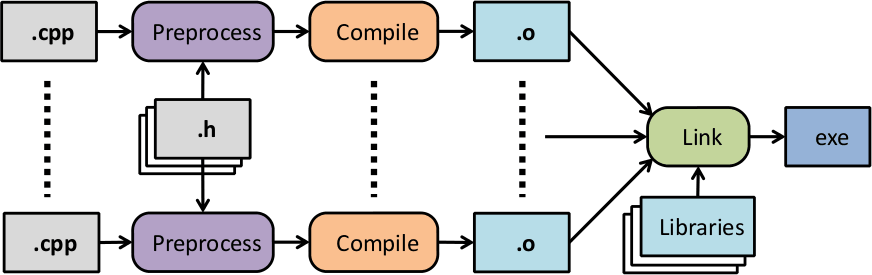
\includegraphics[width=0.75\linewidth]{mainmatter/pics/comp}
	\caption[compiling]{C++ Programm Kompilieren}
	\label{fig:comp}
\end{figure}
\subsubsection{Wozu dieses große Konstrukt?}
Viele Projekte enthalten eine sehr große Menge an Quellcode Dateien. Da man nicht bei jeder kleinen Änderung alle cpp Dateien neu in Objekt Dateien umwandeln will. Kann man auch schlicht nur die geänderten cpp Dateien durch den Preproccesor jagen und anschließend alle .o Dateien neu zu verlinken um die Änderungen zu testen. \\
Außerdem können vorhandene doppelte \#includes verhindert werden, indem man diese mit Guards definiert. Diese verhindern, dass die header Dateien, selbst bei mehrfacher Verlinkung, mehrfach in den Code einkopiert werden. \newpage
\begin{lstlisting}[language=C++]  
//Datei: foo.h
#ifndef A_H
#define A_H
struct foo {
int member;
};
void f(foo&);
...
#endif
\end{lstlisting}
Selbst wenn man nun die foo.h header Datei in mehreren Dateien included, wird sie lediglich einmal hinzugefügt. Denn der Preprocessor, erkennt alle mit \# markierte Zeilen als seine an und führt das if entsprechend der Definition aus. Dabei geht der Guard von \#ifndef A\_H bis \#endif. Das \#define bedeutet, wenn A\_H noch nicht definiert wurde, definiere diese wie folgt. \\
\subsection{Wie lauten die Terminal Befehle dafür?} 
Die Terminal Befehle lauten wie folgt. 
\begin{lstlisting}[language=bash]
g++ -c source.cpp 
g++ -c dbl.cpp 
g++ source.o dbl.o -o test 
\end{lstlisting}
Mit dem Parameter -c werden die angegebenen cpp Dateien in Object Files umgewandelt. Danach linkt man die Object Files mit Hilfe des Parameters -o. Man kann auch direkt -o verwenden wenn man die Dateien direkt in eine .exe Datei umwandeln will.\\
Um das Kompilieren zu vereinfachen, benutzt man bei vielen Dateien eine Makefile. Einen solche sieht wir folgt aus. 
\begin{lstlisting}[language=bash]
#name test
#comment
#compile main 
main.o : main.cpp 
g++ -c main.cpp 
#compile other 
other.o : other.cpp 
g++ -c other.cpp 
#link 
prog: main.o other.o 
g++ main.o other.o -o prog 
\end{lstlisting}
Der Aufruf der Makefile läuft folgendermaßen
\begin{lstlisting}[language=bash]
make test
./prog 
\end{lstlisting}
Mit ./ führt man die generierte .exe aus.
\newpage 
\section{Basics}
\subsection{Variablen}\qquad\\
\begin{itemize}
	\item fängt mir a-z oder \_ an.
	\item enthält a-z, A-Z, 0-9,\_
	\item darf \textbf{nicht} mit einer Zahl beginnen. 
	\item enthalten Werte eines festen Typs.
	\item muss deklariert werden, bevor diese verwendet werden kann. Am besten direkt mit einem Startwert deklarieren.
	\item nach Konventionen, muss die Variable mit einem kleinen Buchstaben beginnen. 
\end{itemize}
\subsection{Arithmetische Operatoren}
\begin{itemize}
	\item + Addition
	\item += Addition mit Zuweisung
	\item - Subtraktion
	\item -= Subtraktion mit Zuweisung
	\item * Multiplikation
	\item *= Multiplikation mit Zuweisung
	\item / Division
	\item /= Division mit Zuweisung
	\item \% Modulo
\end{itemize}
\subsection{Increment / Decrement}
\begin{tabular}{ccc}
	& prefix & postfix \\ 
increment	& ++a & a++  \\ 
decrement	& --a & a-- \\ 
\end{tabular} \\\qquad \\
Der Unterschied zwischen prefix und postfix ist, dass bei einer Zuweisung wie
\begin{lstlisting}[language=C++] 
a = ++b;
\end{lstlisting}
der Wert von b erst erhöht wird und danach erst zugewiesen wird. Bei 
\begin{lstlisting}[language=C++] 
a = b++;
\end{lstlisting}
wird der Wert erst zugewiesen und daraufhin erhöht. 
\subsection{Typen}
\begin{figure}[h]
\centering
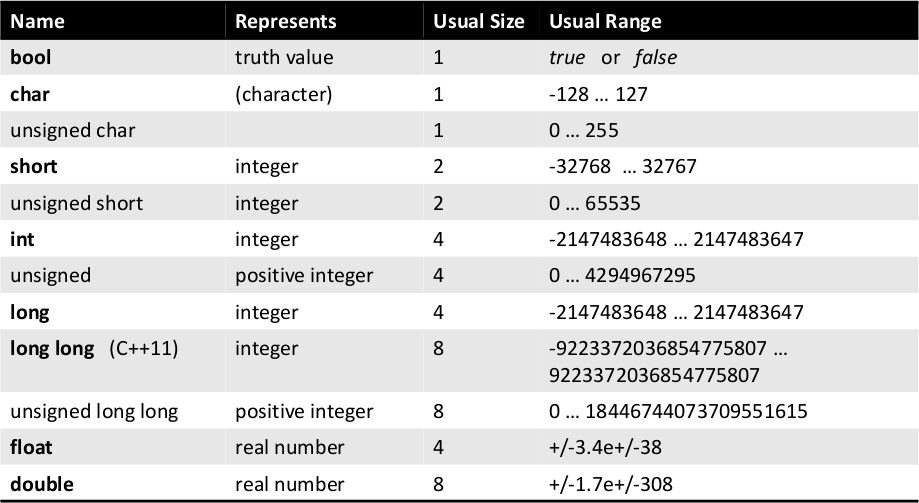
\includegraphics[width=0.75\linewidth]{mainmatter/pics/typ}
\caption[typen]{Alle Typen im Überblick}
\label{fig:typ}
\end{figure}
Jedoch gilt es zu beachten das long und int meist gleich lang sind auf 32Bit Systemen und das der C++ Standard lediglich die Minimale Größe Garantiert.
\subsection{Logik Operationen}\qquad\\
\&\& / and = Und\\
|| / or = Oder\\
! / not = Negation\\
0 = false\\
alles $\neq$ 0 = true
\subsection{Vergleiche}
== ; < ; > ; >=; <= ; !=
		
\subsection{Funktionen}
\begin{lstlisting}[language=C++]
return_type name (parameters) {
	//body
}
\end{lstlisting}
Die Main Funktion wird mit dem return\_type int versehen, da Programme in der Regel eine 0 zurückliefern, sofern diese ohne Probleme durchgelaufen sind. \\
Eine Funktion darf lediglich einen Rückgabewert enthalten. Um sich mehrere Rückgabewerte zu generieren bedient man sich eines Tricks, dieser heißt Call by Reference$^{\ref{sec:call}}$.Dadurch arbeitet man auf den Variablen außerhalb der Methode.\\ 
Alle in der Main benutzten Methoden müssen vor der Main bereits bekannt sein. Dies kann man erreichen, indem man alle Funktionen bereits vor der Main definiert, oder diese vorher definiert und später mit leben füllt.\\
\begin{lstlisting}[language=C++]
void odd (int a);

int main ()
{
	int i;
	do {
		cout << "Type a number: ";
		cin >> i;
		odd (i);
	} while (i!=0);
}

void odd (int a)
{
	if ((a%2)!=0)
	cout << "Number is odd.\n";
.
.
.
.
\end{lstlisting}
Um Standard Parameter zu nutzen, (also Parameter, welche einen Wert haben, ohne übergeben worden zu sein.) muss man bei der Parameterliste diese initialisieren.
\begin{lstlisting}[language=C++]
//Beispiel 1:
float mulf(float a, float b = 1.5f) { 
	return (a * b); 
} 
//Beispiel 2:
float mulf(float a, float b = 1.5f, float c) { 
	return (a * b * c); 
} 
\end{lstlisting}
Beispiel 1 funktioniert wie erwartet, jedoch wird Beispiel 2 nicht funktionieren, da die Variable c nicht initialisiert ist, obwohl diese nach einer bereits initialisierten kommt. \\
\subsubsection{Überladen}
\begin{lstlisting}[language=C++]
int abs (int i) {
	return ((i < 0) ? -i : i);
}
float abs (float i) {
	return ((i < 0) ? -i : i);
}
double abs (double i) {
	return ((i < 0) ? -i : i);
}
//----------------------------
int foo (int i) {
	return (2 * i);
}
double foo (int i) {
	return (2.5 * i);
}
//-----------------------------
int foo (int i, int k = 2) {
	return (2 * i * k);
}
int foo (int i, int k = 2, int l = 3) {
	return (2 * i * k * l);
}
\end{lstlisting}
Das was im ersten Abschnitt steht funktioniert einwandfrei. Genau so sollte an Funktionen überladen.\\
Der zweite Abschnitt funktioniert nicht, da nicht nur der Rückgabewert geändert werden kann, sondern auch die Parameterliste verändert werden muss. \\ 
Das Beispiel aus dem dritten Abschnitt funktioniert nicht wie erwartet. Denn der Compiler muss wissen können, welche Funktion er nimmt. Wenn man nun foo(3) aufruft, kann der Compiler nicht entscheide, welche der Funktionen genutzt wird. 

\section{Kommandozeilen Argumente}\label{sec:kommando}
Hier ein kleines Beispiel, wie man Kommandozeilen Argumente beim Start eines Programmes direkt übergibt, ausliest und auf der Konsole ausgibt. 
\begin{lstlisting}[language=C++]
#include <iostream>

using namespace standard

int main(int argc, char* argv[])
{
for(int i = 1; i<argc;++i){
cout << argv[i] <<endl;
}
return 0;
}
\end{lstlisting}
\begin{lstlisting}[language=Bash]
> ./test 12 3 abc def
test
12
3
abc
def
\end{lstlisting}
argc und argv sind nur Konventionen und können anders benannt sein. argc enthält die Anzahl der Elemente und argv ist ein C Array. Die Elemente von argv sind wiederum C Strings.  
\section{I/O from console/file}	\qquad\\
Damit das Programm auch von einem Benutzer gesteuert werden kann, Reichen meist die Kommandozeilenparameter$^{\ref{sec:kommando}}$ nicht aus. 
\subsection{I/O from console}\qquad\\
Damit der Benutzer während des Programmablaufs Daten eingeben kann, fordert man ihn über die Konsole zu einer Eingabe auf. 
\begin{lstlisting}[language=C++]
#include <iostream>
using namespace std;
int main(){
	int i = 0;
	cout << "Geben Sie eine Zahl ein" << endl;
	cin >> i ; 
	cout << "Sie haben " + i + " eingegeben" << endl;
}
\end{lstlisting}
\#include <iostream> ermöglicht es Text von der Kommandozeile zu lesen und in dieser wiederzugeben.\\
using namespage std; ermöglicht es cout, cin und endl; so abgekürzt zu schreiben. 
\subsection{I/O from File}
Um mit größeren Datenmengen zu arbeiten ist es Sinnvoll Dateien auslesen zu können. Dies kann man z.B. mit folgendem Programm machen. 
\begin{lstlisting}[language=C++]
#include <fstream>
using namespace std;
int main(){
	// Datei lesen
	ifsteam datei ("file.txt");
	if (datei.is_open()){
		while (!datei.eof()){
			string s;
			getline(datei,s);
			cout << s << endl;
		}
	}
	datei.close();
	// Datei schreiben
	ofstream output ("file_copy.txt");
	if (output.is_open()){
		for (int i = 0; i < 20; ++i){
			double i2 = i*i;
			output << i << '\t' << i2 << '\n';
		}
	}
	output.close();
	return 0; 
}
\end{lstlisting}
Um Dateien zu öffnen gibt es unterschiedliche Modi. 
\begin{itemize}
	\item Default:
	\begin{itemize}
		\item ifstream is("in.txt", ios::in);
		\item ofstream os("out.txt", ios::out);
		\item allow input / output operations
	\end{itemize}
	\item Append:
	\begin{itemize}
		\item ofstream os("log.txt", ios::app);
		\item each insertion is done at the stream end
	\end{itemize}
	\item Binary:
	\begin{itemize}
		\item ifstream is("pic.jpg", ios::binary);
		\item ofstream os("pic.jpg", ios::binary);
		\item consider stream as binary (rather than text)
	\end{itemize}
\end{itemize}

\section{Control Statements and Loops}
\subsection{if .. then .. else / Switch}
\begin{lstlisting}[language=C++]
if (condition1) {
	//do this if condition1 is true
}
else if (condition2) {
	//otherwise do this if
	//condition2 is true
}
else {
	//otherwise do this 
}
\end{lstlisting}
\qquad\\
\begin{lstlisting}[language = C++]
switch(m){
	case 0:
		//do this if 0
		break;
	case 1:
		//do this if 1 and got to the next 
		//cause of missing break
	case 3: 
		//do this if 3
	break;
	default:
		// if everything else fails do this	
}
\end{lstlisting}
Für das m im switch können char, int, long und weitere Zahlenwerte verwendet werden. 

\subsection{Loops}
\begin{lstlisting}[language=C++]
for (int i = 0; i < 5; ++i) {
cout << i << endl;
}

int j = 5;
while (j < 10) {
cout << j << endl;
++j;
}

do {
cout << j << endl;
--j;
} while (j > 0);
\end{lstlisting}	
\section{Call by Value / Call by Reference}\label{sec:call}
\begin{lstlisting}[language=C++]
// Call by Value
int foo(int n) { 
n += 10; 
return (2 * n); 
} 
// Call by Reference 
int bar(int& n) { 
n += 10; 
return (2 * n); 
} 
int main()
{
int i = 10;
cout << foo(i) <<" "<< i << endl; //Ausgabe 40 10
cout << bar(i) <<" "<< i << endl; //Ausgabe 40 20
return 0;
}
\end{lstlisting}
Bei Call by Value wird eine Deep Copy angelegt von dem Wert. Der Wert wird kopiert und mit dieser Kopie wird in der Methode gearbeitet. \\
Bei Call by Reference wird der Wert als Referenz übergeben. Dadurch wird der wert außerhalb der Funktion verändert. Durch diesen Trick kann man sich z.B. mehrere Rückgabewerte erstellen.\\
\textbf{!!Achtung!!} Wenn eine Referenz als Argument erwartet wird, kann keine Zahl direkt übergeben werden. Lediglich Variablen welche auf den Wert referenzieren, oder diesem direkt zugewiesen sind.
\section{Pointer und Referenzen}
\subsection{Referenzen}
Referenzen referenzieren einen Wert lediglich. Wenn man den Wert einer Referenz ändert, so ändert man den Wert der Variable auf den die Referenz zeigt. Dies ist nützliche, da man Werte als Referenzen an eine Methode übergeben kann. Dadurch hat man die Möglichkeit sich mehr als einen return Wert zu generieren. Da man die Variable außerhalb der Methode ändert und nicht nur die Unbekannte innerhalb der Methode. \\
\begin{lstlisting}[language=C++]
// Initialisierung
int i = 2;
int& ri = i; 
const int& ci = i;
double& blub = i; // => Fehler da die Typen identisch sein muessen.
int& rj; // Fehler, da Referenzen immer initialisiert sein muessen

// Wertzuweisung
i = 5; // i, ri, ci geben den Wert 5 aus
ri = 6; // i, ri, ci geben den Wert 6 aus
ci = 88 // Fehler, da ci als const definiert wurde und nicht geaendert werden kann. 
\end{lstlisting}
Mit int\& i erstellt man eine Referenz. Mit \&i bekommt man die Speicheradresse der Variable i. 
\subsection{Pointer}
Pointer sind Variablen, die auf eine Speicheradresse verweisen. Sie verweisen nie direkt auf einen Wert. 
\begin{lstlisting}[language=C++]
int a, b; //two ints
int* p; //a pointer to an int
p = &a; //nehme Speicheradresse von a und Speichere diese in p
*p = 10; //Dereferenziere p und veraendere den Wert.
p = &b;
*p = 20;
cout << a << endl; //10
cout << b << endl; //20
\end{lstlisting}
\subsection{Stolperfallen}
\begin{lstlisting}[language=C++]
int* p1, p2; // int pointer, int
int *p1, *p2; // int pointer, int pointer
//better
int* p1; //int pointer
int* p2; //int pointer
int* p = nullptr; // nullptr, sollte die Standard initialisierung sein. 
//Damit der Pointer nicht mit irgendwelchen Werten initialisiert ist. 
\end{lstlisting}
Pointer können hochgezählt werden wie normale integer. Denn der Wert der im Pointer steht ist lediglich eine Speicheradresse, also eine Zahl. Mit jedem p++ springt man um so viele Speicherstellen weiter, wie p groß ist. 
\begin{lstlisting}[language=C++]
int v = 5; 
int* p = &v; 
int** pp = &p;
 
cout << v; // 5
cout << p;  // 0x40
cout << pp; //0x44

cout << &v; //0x40 (= p)
cout << &p; //0x44 (= pp)
cout << &pp; //0x48

cout << *p;  //5
cout << *pp;  //0x40 (= p)
cout << **pp;  //5
\end{lstlisting}
Da Array Bezeichner gleichzusetzen sind mit einen Pointer auf den ersten Wert des Arrays, kann man Arrays genauso behandeln. Mann kann Arrays in Funktionen als Pointer übergeben,(dabei sollte man die Größe des Arrays mit übergeben.) und diese hoch zählen um zum nächsten Element zu kommen oder auch Addition ausführen um eine Variable an einer bestimmten Stelle zu bekommen. Wenn man mit dem Wert in einer Funktion arbeiten will, muss man den Pointer dereferenzieren, ansonsten arbeitet man dort mit der Speicheradresse. \\

\begin{figure}[h!]
\centering
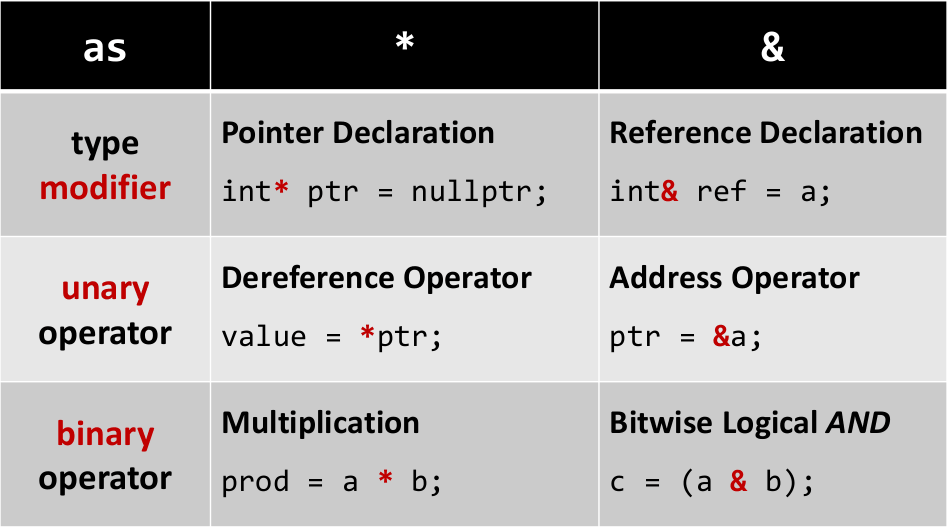
\includegraphics[width=0.6\linewidth]{mainmatter/pics/syn}
\caption[Pointer/Referenzen Syntax]{Pointer/Referenzen Syntax}
\label{fig:syn}
\end{figure}
\begin{figure}[h!]
\centering
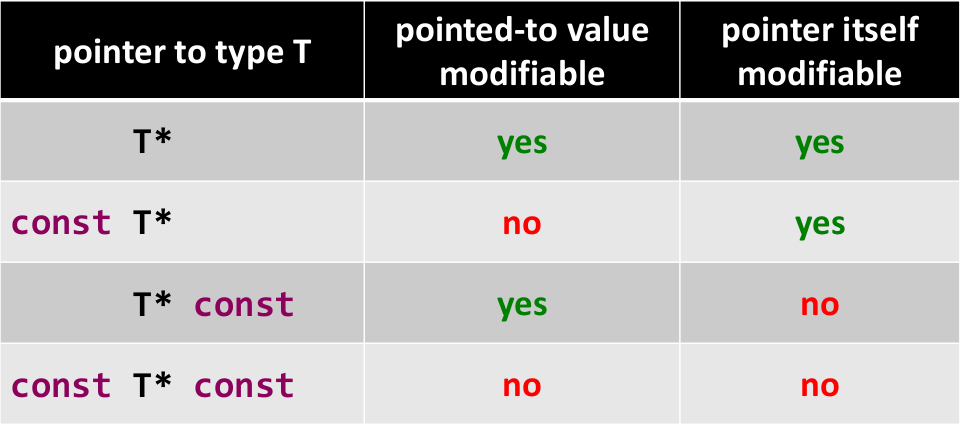
\includegraphics[width=0.6\linewidth]{mainmatter/pics/pconst}
\caption[const Pointer]{const Pointer}
\label{fig:pconst}
\end{figure}
\begin{figure}[h!]
\centering
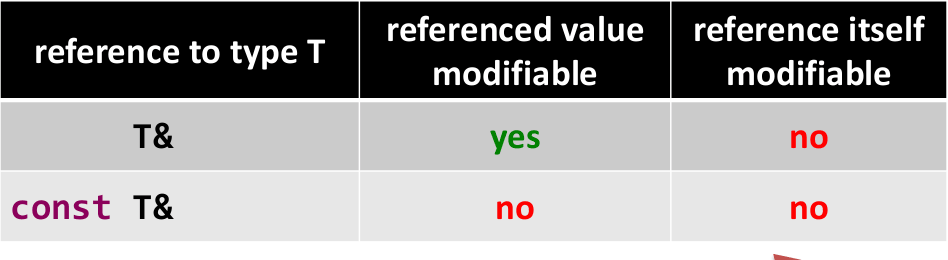
\includegraphics[width=0.6\linewidth]{mainmatter/pics/rconst}
\caption[const Referenzen]{const Referenzen}
\label{fig:rconst}
\end{figure}
\newpage

\section{Memmory Management (Stack/Freestore)}
\subsection{Stack}
\begin{itemize}
	\item sequentieller Speicher von vordefinierter Größe
	\item zusammenhängender Speicher
	\item wird für lokale Variablen benutzt
	\item automatisches Speichermanagement
	\item last in first out
	\item für gewöhnlich lediglich ein paar MB groß
	\item STack wurde für lokale Variablen und Parameter 
\end{itemize}
Im Stack werden die einzelnen Variablen angelegt, sobald sie definiert werden.  Wird eine Funktion aufgerufen, wird eine Return Adresse auf den Stack gelegt. Also wohin das Programm  zurück springen muss, wenn die Funktion abgearbeitet ist. Darauf wird der Return Value im Speicher gelegt, sofern es einen gibt, dieser dient als Platzhalter für den Wert der Variable. Sobald die CPU in der nächsten Funktion ist wir ein Stack Frame angelegt, dieser ist eine Art Markierung auf dem Stack, bis wohin die nun kommenden Variablen gültig sind. Als erste Werte werden die Funktionsparameter auf dem Stack abgelegt. Wenn die Funktion beim return ankommt, wird dieser Value in den Placeholder (RV) geschrieben und der Stack wird bis einschließlich dem StackFrame frei gegeben, jedoch nicht gelöscht und die CPU spring zur Return Adresse. \\
\textbf{!!ACHTUNG!!} Wenn man eine Referenz zurück gibt, wird versucht diese aus dem Stack zu lesen, was nicht funktioniert, da diese Variable bereits frei gegeben wurde. Wenn man Glück hat, und keine Funktion zwischenzeitlich den Wert überschrieben hat, bekommt man den passenden Wert ansonsten einen vorher nicht definierten. Daher sollte man immer den Wert zurück geben, da der Stack von jeder Funktion überschrieben werden kann.  
\subsection{FreeStore (Heap)}
\begin{itemize}
	\item großer Speicher Bereich (der größte Teil des RAM's)
	\item muss nicht zusammenhängend sein. 
	\item wird benutzt um dynamisch Speicher zu allozieren
	\item manuelles Speichermanagement.
	\item Operator new alloziert ein neues Element im FreeStore 
	\item Operator delete gibt den Speicher des Elements im FreeStore frei.
	\item dort angelegte Variablen / Objekte etc. leben so lange wie notwendig.
\end{itemize}
\begin{lstlisting}[language=C++]
Type* p = new Type(args...); //create new variable of type "Type"
Type* a = new Type[s] //create new C-array of size s of type "Type"
delete p; //free variable p
delete[] a; //free C-array a (square bracket syntax)
\end{lstlisting}
\subsubsection{Fallstricke und wie man diese umgeht}
\begin{itemize}
	\item nicht instantiierte Pointer können alles mögliche enthalten.
	\item der Programmierer muss sicherstellen, dass die Pointer instantiiert sind. Am besten mit nullptr .
	\item bei Übergabe von Pointer diese immer auf nullptr testen.
	\item wenn die Elemente im Pointer gelöscht werden, sollte der Pointer auf nullptr gesetzt werden.
\end{itemize}
\section{Structs}
\section{Complex Data Structures (Lists, Trees)}
\section{Standard Containers and Algorithms}	

